\section*{\Huge Design}
\addcontentsline{toc}{chapter}{Design}
\markright{Design}

% --------------------
\section{Design Considerations}

\textbf{Assumptions}

1. \textbf{Database Access and Format}: We assume that our proposed system should ideally have access to all target databases in the environment in which it is deployed, and such that they are accessible and follow standard SQLite format with full READ access that grants programmatic inspection permissions. It directly relates to our requirements as follows:
\begin{itemize}
    \item \textbf{Functional}: Enables schema retrieval, column exploration, and dialect-specific SQL generation. Without READ access and column exploration, the retrieval and query planning stages would fail.
    \item \textbf{Non-Functional}: Ensures reproducibility and correct execution on the Spider 2.0-Lite benchmark. Accessibility allows preprocessing (e.g., RAG index construction) and supports handling enterprise-scale schemas (up to 1000 columns) in our benchmark.
    \item \textbf{Resource}: Evaluation is planned only on Spider 2.0-Lite (SQLite) and upcoming benchmarks like BEAVER are being considered for capability estimation of our architecture. The above design should avoid additional data annotation or integration efforts.
\end{itemize}

2. \textbf{Natural Language Input}: Queries are assumed to be in English, and unambiguous enough for the system schema exploration tools to extract meaningful context. Its impact on our design concept:

\begin{itemize}
    \item \textbf{Functional}: The system can safely perform query rewriting, planning, and SQL generation stages. Input validation and actionable feedback (in query correction loops) rely on this assumption.
    \item \textbf{Non-Functional}: Supports (nearly) deterministic execution accuracy and reproducibility. Unpredictable or non-English queries could lead to failures and/or degraded accuracy.
    \item \textbf{Resource}: Minimizes the need for multi-language embeddings or additional preprocessing pipelines.
\end{itemize}

3. \textbf{Agent Reliability}: Using a single large model across all reasoning stages significantly increases inference cost without proportional accuracy gains. As per our intermediate proposal, each sub-agent component like the discovery agent, debate-consensus agent, SQL planner, self-correction agent operates correctly and communicates reliably within the system pipeline. This is interrelated to our requirements and it impacts our design concept and operations:

\begin{itemize}
    \item \textbf{Functional}: Critical for enabling the iterative self-correction loop, SQL validation, and error analysis. Each stage depends on the previous stage for producing valid output.
    \item \textbf{Non-Functional}: Supports high-accuracy and low-latency performance (not our primary goal). It can also help ensure transparency through reliable logging of intermediate artifacts (plans, retrieved context, correction iterations).
    \item \textbf{Resource}: Justifies modular architecture design, enabling independent development and configuration of agents without redundant computation or failure handling overhead.
\end{itemize}

We plan to assign lightweight models for execution validation and correction experimentation, and stronger reasoning models for planning and decomposition. This maintains a high execution accuracy while controlling token usage during large-scale benchmark evaluation. The current architecture is explicitly optimized for iterative reasoning loops, schema exploration calls, multi-agent consensus strategies, that may not look completely production ready, but they are important for a top-tier leader board performance.

\textbf{System Environment, Constraints, and Design Methodology}

1. \textbf{Schema Retrieval with Vector-Based Filtering}: Embedding-based schema retrieval supports the requirement that the system can accurately handle enterprise-scale schemas. By filtering irrelevant tables before planning, the system reduces context overload and improves column selection accuracy. With respect to our benchmark, naïve full-schema prompting is infeasible within LLM context limits. Existing leaders on the leaderboard such as Databao \cite{jetbrains2026databao} rely primarily on static schema summarization or shallow retrieval, which often leads to missing relevant columns in nested or compositional queries. To address this limitation, our design prioritizes:
    \begin{itemize}
        \item vector-based schema retrieval before planning,
        \item column-level semantic ranking,
        \item dynamic schema exploration during reasoning.
    \end{itemize}

    This should ensure our architecture system maintaining high recall of relevant schema elements while remaining within context window constraints.

2. \textbf{Explicit Query Planning Stage}: The query planning module supports the functional requirement that the system should generate structured intermediate reasoning artifacts prior to SQL synthesis. A key weakness is conduction direct SQL synthesis without a sufficiently explicit intermediate reasoning structure. Although syntax errors can often be corrected iteratively, logical errors propagate across correction loops and reduce execution accuracy. To mitigate this, our architecture introduces an explicit query planning stage that decomposes complex questions into sub-tasks, identifies join paths using schema structure, and determines aggregation and filtering strategy before generation. Structured planning should also improve our robustness for nested queries and compositional reasoning tasks.

3. \textbf{Multi-Path Candidate SQL Generation}: Generating multiple candidate SQL queries satisfies the execution-accuracy requirement of achieving performance above 55\% on Spider 2.0 Lite. Single-path generation pipelines are sensitive to early reasoning mistakes. In competitive architectures like Databao, sequential correction loops are used in sync with their context engine rather than exploring alternative reasoning trajectories.

Our system instead adopts a multi-path candidate generation strategy where we intend to generate multiple SQL candidates are generated from different reasoning paths, have voter agents evaluate candidates, and then select the best query for execution. Or, we may involve sub-agent tasks as detailed previously. But overall, our combined goal is to increase resilience to early-planning errors.

4. \textbf{Semantic Self-Correction Loop}: Extending corrections beyond syntax repair supports the requirement that the system recover from logical execution failures using database feedback. This directly improves convergence reliability during iterative refinement.

We design our correction loop to include semantic validation through lightweight execution probes, schema-aware reasoning feedback, and backtracking to earlier planning stages when necessary. Our aim to enable recovery from logical errors, surface-level failures and distinguishing between both.


\section{System Architecture/Design Overview}

Our NL2SQL system architecture follows a structured pipeline where valid natural language questions are progressively transformed into validated SQL queries through context enrichment, intelligent planning, distributed execution, and systematic merging. It is a modular, multi-agent pipeline that is capable of decomposition, contextual grounding, and iterative self-correction.
At a high level, the system consists of four primary stages: Preprocessing, Planning, Execution of Sub-tasks (via Sub-agents), and Merging \& Validation. Each stage is composed of well-defined components that interact through structured inputs and outputs.

\begin{enumerate}
    \item \textbf{Preprocessing Layer}: This stage constructs the foundational context required for downstream reasoning. We are currently iterating on two key modules:
    
    a. \textbf{Knowledge Graph}: The Knowledge Graph should enrich the structural and semantic relationships within the database schema. It includes: 
    - Foreign key relationships for join path discovery. Join path candidates across tables and column-level value distributions and profiles. We are trying to include term aliases and semantic mappings for schema elements. Overall, our goal is to enable schema-aware reasoning and reduce ambiguity in query construction.

    b. \textbf{Context Engine}: The Context Engine retrieves and organizes relevant schema information using hybrid search techniques. It provides:
    - Schema chunks (table and column groupings) that have column descriptions and metadata.
    - Contextual retrieval based on the input question.
    Together, these components ensure that the system operates with a grounded and query-relevant view of the database.

\begin{figure}[H]
    \centering
    \includegraphics[width=1.0\linewidth]{MCDS-Capstone-Planning-Report-Template/diagrams/high-level.png}
    \caption{High-level architecture diagram showing the Preprocessing Layer, Planner Agent, Subagent Execution Layer, and Merger Agent.}
    \label{fig:erd}
\end{figure}

    \item \textbf{Planner Agent}: The Planner Agent is responsible for transforming the input natural language question into a structured decomposition plan. There is an input component which uses the NL question and the preprocessed schema context. It outputs a decomposition plan consisting of ordered sub-tasks via explicit reasoning "thinking stage", by breaking the problem before SQL generation, improving interpretability and modularity. It is able to:
    
    - Identify required tables and join paths
    
    - Detect potential null-value edge cases
    - Infer table shapes and aggregation requirements
    
    - Break down complex queries into smaller, manageable sub-tasks


\begin{figure}[H]
    \centering
    \includegraphics[width=0.7\linewidth]{MCDS-Capstone-Planning-Report-Template/diagrams/low-level.png}
    \caption{A detailed architecture diagram showing the interconenctions among the four major modules: Preprocessing Layer, Planner Agent, Subagent Execution Layer, and Merger Agent}
    \label{fig:erd}
\end{figure}

    \item \textbf{Subagent Execution Layer}: We have designed the system to employ multiple specialized Sub-agents, each responsible for solving an individual sub-task derived from the planner. It should generate SQL queries for specific sub-tasks and operate independently but consistently within the global plan. It has some tools available to it namely: Knowledge Graph (for relational reasoning) and the Context Engine (for schema grounding) which it uses along with Sub-task specification. 
    Our parallelized design enables scalability and isolates errors to specific components, making debugging and optimization more tractable.

    \item \textbf{Merger Agent}: The Merger Agent integrates the outputs of all sub-agents into a single coherent SQL query and ensures correctness. It should produce the final executable SQL query and result, verify and synthesize to ensure that independently generated components form a logically consistent and correct query. 
    
    It incorporates subagent-generated SQL queries, the original NL question and the decomposition plan to:
    
    - Validate individual subqueries (e.g., via test execution of CTEs)
    
    - Resolve inconsistencies or conflicts across subqueries

    - Compose a final query using structured constructs such as WITH clauses (CTEs)
    
    - Perform result validation against expected semantics

    
\end{enumerate}

\section{Data Design}

\subsection{Raw SQLite Databases}

The source data for both the Context Engine and the benchmark evaluation is drawn from the \textbf{Spider 2.0-Lite} dataset, hosted on GitHub at \texttt{spider-agent/spider2}. The SQLite track provides 32 database files, covering domains such as Baseball, E-commerce, WWE, EU Soccer, F1 Racing, Northwind, Chinook, IMDB Movies, and California Traffic Collision, among others.

Each database is a self-contained \texttt{.sqlite} file ranging from a few MB to over 50 MB (e.g., WWE is 54 MB). No schema documentation or column descriptions are provided - the only available information is the raw table structure, column names, types, and the data itself.

Alongside the databases, the benchmark supplies a task file (\texttt{spider2-lite.jsonl}) where each entry specifies the target database, a natural language question, and an optional external knowledge document. For example:

\begingroup\small
\begin{verbatim}
{
  "instance_id": "local003",
  "db": "E_commerce",
  "question": "Calculate the average sales per order for each customer
               within distinct RFM segments...",
  "external_knowledge": "RFM.md"
}
\end{verbatim}
\endgroup

External knowledge documents  contain domain-specific definitions that the agent must incorporate to answer correctly. These are injected into the agent's context at query time.

\subsection{Context Engine Pipeline}

The Context Engine transforms raw SQLite databases into a searchable vector index through a three-stage pipeline: schema extraction, LLM enrichment, and chunk embedding.

\begin{figure}[H]
\centering
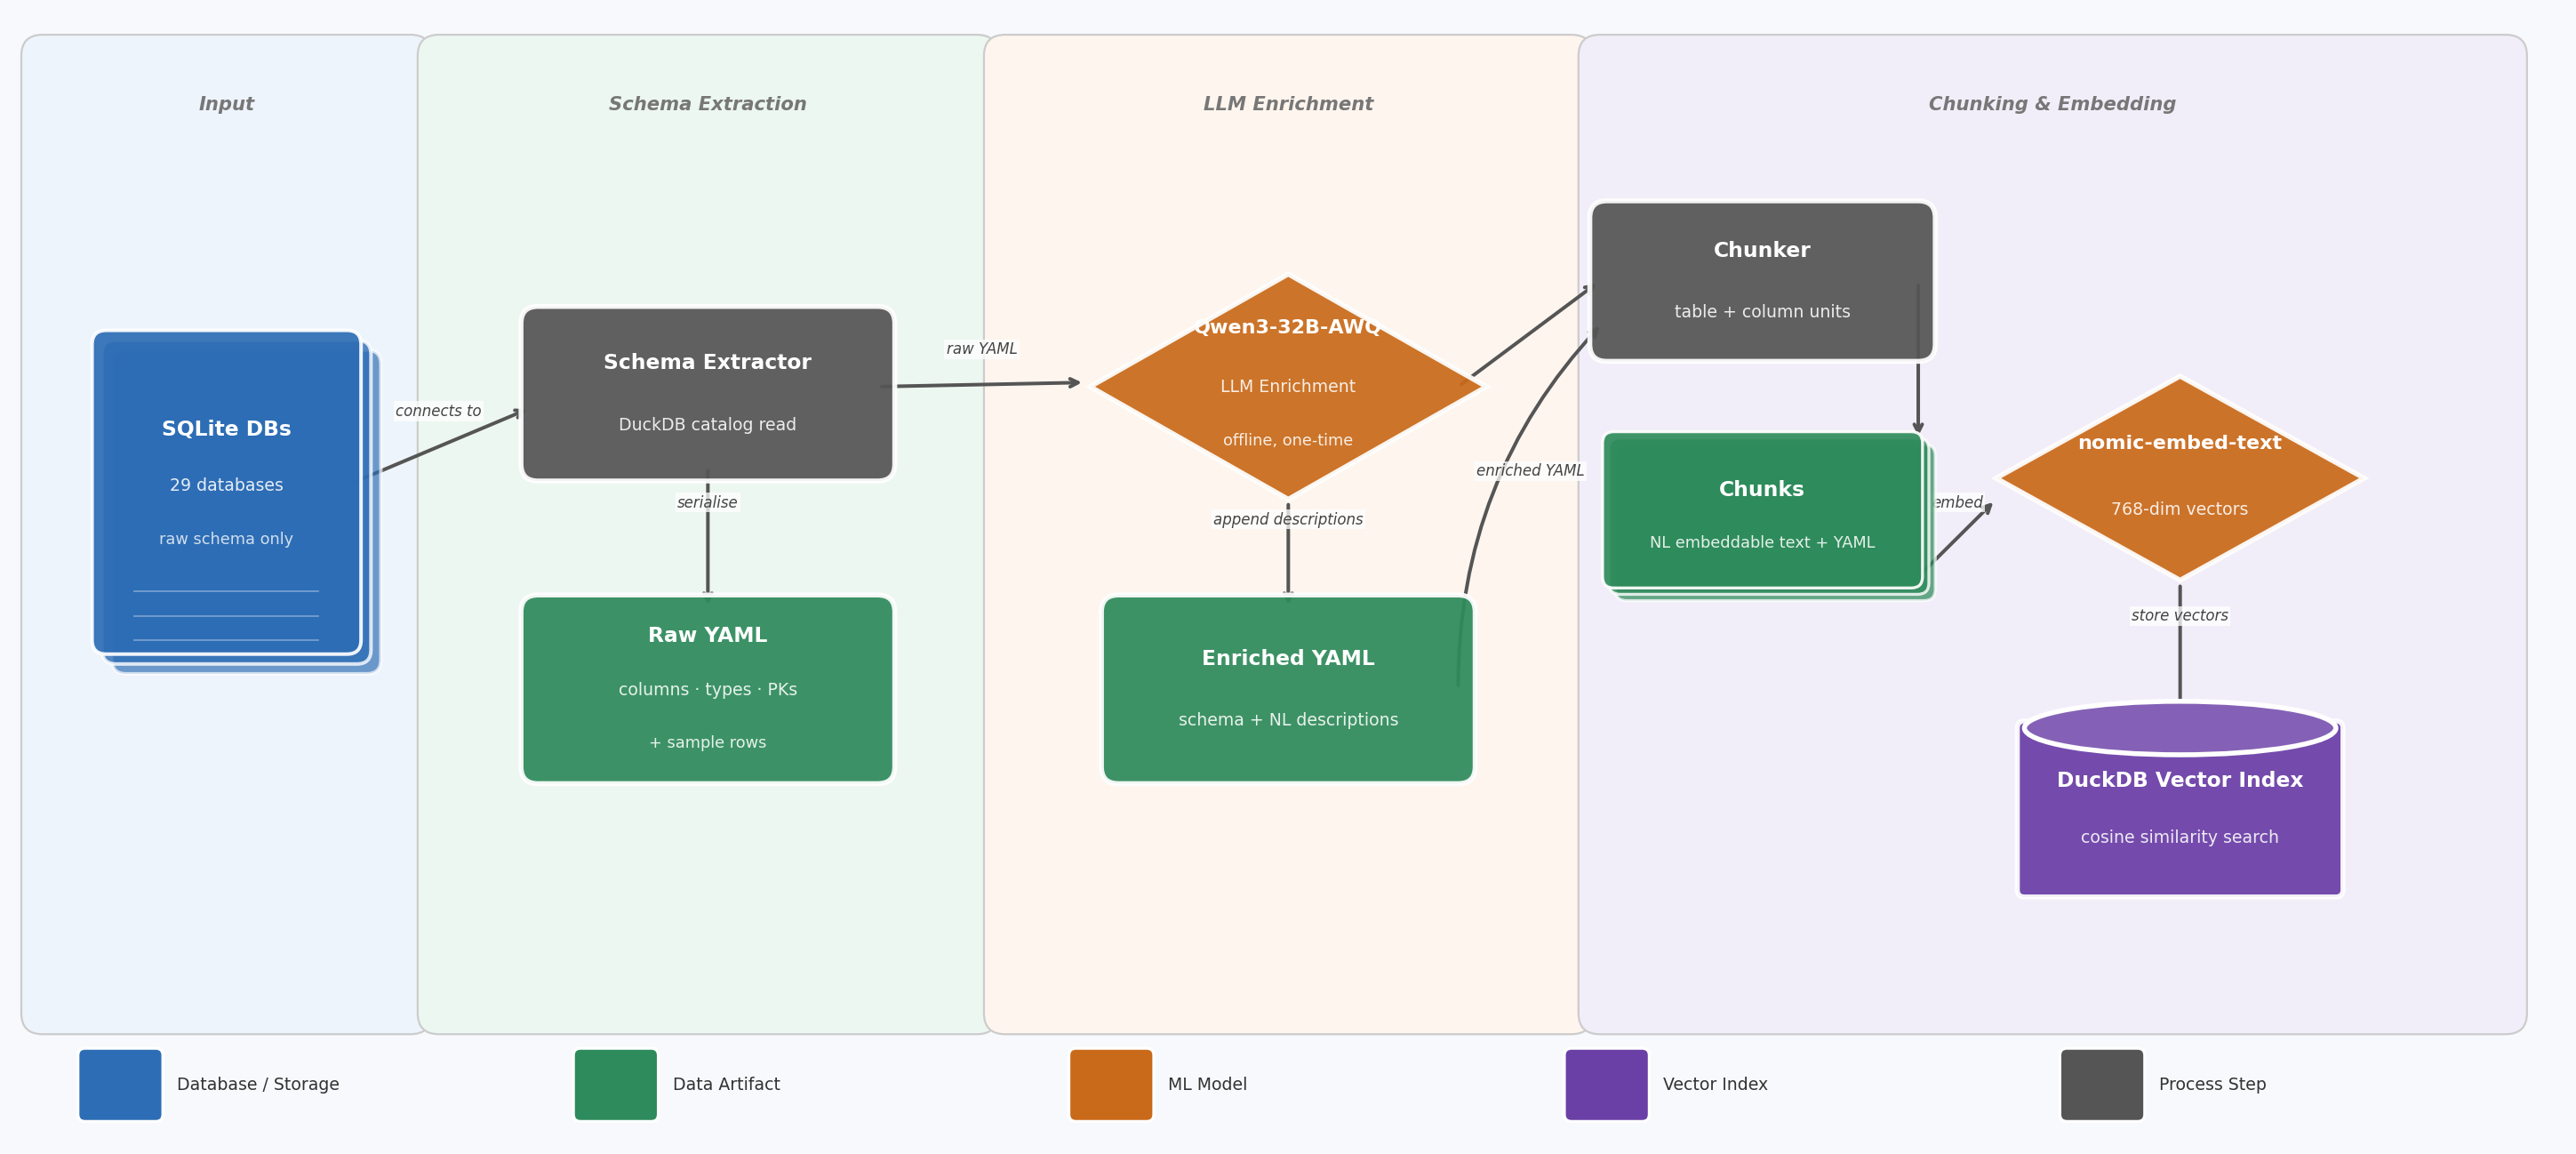
\includegraphics[width=\linewidth]{dce_pipeline.png}
\caption{Context Engine preprocessing pipeline: raw SQLite schema is extracted, enriched with LLM-generated descriptions, chunked into table and column units, embedded, and stored in a DuckDB vector index.}
\label{fig:dce_pipeline}
\end{figure}

\subsubsection{Schema Extraction}

Schema extraction connects directly to each \texttt{.sqlite} file via DuckDB, reading column names, types, nullability, primary keys, foreign keys, and unique constraints from the database catalog. Up to five representative rows are sampled per table. This structural metadata is serialised into a YAML file per database. Each table entry includes the full column list, a primary key declaration, foreign key references, unique constraints, and sample rows. The example below shows the \texttt{Belts} table from the WWE database:

\begingroup\small
\begin{verbatim}
table:
  name: Belts
  primary_key:
    columns: [id]
  columns:
    - name: id
      type: INTEGER
      nullable: false
    - name: name
      type: TEXT
      nullable: true
  samples:
    - {id: 1,  name: ""}
    - {id: 9,  name: "WWWF World Heavyweight Title"}
\end{verbatim}
\endgroup

\subsubsection{LLM Enrichment}

The raw YAML is passed to Qwen3-32B-AWQ, which appends a natural language \texttt{description} field to every table and column entry. These descriptions capture semantic meaning that cannot be inferred from column names or types alone, such as the domain significance of a field or how values are formatted. After enrichment the same entry becomes:

\begingroup\small
\begin{verbatim}
    - name: name
      type: TEXT
      nullable: true
      description: "Stores the belt name as free text."
  description: "Championship belts with unique id and name."
\end{verbatim}
\endgroup

\subsubsection{Chunking into Vector DB}

The enriched YAML is split into two chunk types before embedding:

\begin{itemize}
  \item \textbf{Table chunk} - one per table. The \emph{embeddable text} (used for similarity search) is a natural language sentence summarising the table: its column count, primary key, and column list. The \emph{display text} (returned to the agent) is the full enriched YAML block for that table, including samples and descriptions.
  \item \textbf{Column chunk} - one per column. The embeddable text describes the column type, nullability, and any PK/FK role. The display text is the YAML snippet for that column with its LLM description.
\end{itemize}

Concrete examples from the WWE \texttt{Belts} table:

\begingroup\small
\begin{verbatim}
-- Table chunk (embeddable text):
"Belts is a database table with 2 columns.
 Primary key: id (INTEGER). Columns: id, name"

-- Column chunk (embeddable text):
"name is a column of type TEXT in table Belts.
 Nullable. Stores the belt name as free text."
\end{verbatim}
\endgroup

Both chunk types are embedded with \textbf{nomic-embed-text-v1.5} (768-dim) and stored alongside their display text in a DuckDB table. At query time, the agent issues a natural language query which is embedded and compared against all chunks via cosine similarity; the top-$k$ display-text YAMLs are returned for the agent to reason over.

\subsection{Benchmark Data}

The same 29 databases loaded into the Context Engine are the evaluation targets for the Spider 2.0-Lite SQLite benchmark. Each benchmark question is paired with one database; the agent answers using only that database's schema and any external knowledge document supplied by the benchmark. A representative question from the Baseball database is:

\begin{quote}
\textit{``Calculate the average career span in years for all baseball players, where career span = ROUND(years, 2) + ROUND(months/12, 2) + ROUND(days/365, 2), and years/months/days are the calendar components of the difference between debut and final game dates.''}
\end{quote}

The agent's SQL result is executed against the database and compared to a pre-computed gold CSV; a question is counted correct only if the result matches within the defined tolerances (see Section on Test Design).

\section{Implementation Overview} \label{sec:design_sec4}
% Include an overall workflow diagram that clearly shows how your system is intended to operate at the module level; you may include, as necessary:
% \begin{itemize}
%     \item A domain model (e.g., UML, ERD, etc.);
%     \item A dataflow diagram for the overall system or for each use case (e.g., UML sequence diagrams);
%     \item Component design: UML package diagrams, UML static structure diagrams, Javadoc APIs;
%     \item Interface design: site maps, screenshots, storyboards, service APIs;
%     \item Activity/Entity/Class/Sequence Diagrams
% \end{itemize}


\begin{figure}[H]
    \centering
    \includegraphics[width=1.0\linewidth]{MCDS-Capstone-Planning-Report-Template/diagrams/domain_model.png}
    \caption{Domain class diagram showing the decomposition of a UserQuery into SubTasks, SQL fragments, and the final assembled SQL}
    \label{fig:erd}
\end{figure}

\begin{figure}[H]
    \centering
    \includegraphics[width=1.0\linewidth]{MCDS-Capstone-Planning-Report-Template/diagrams/sys_flow.drawio.png}
    \caption{System dataflow showing query decomposition by the Planner Agent, parallel subagent execution, and CTE merging}
    \label{fig:sys_diag}
\end{figure}

\begin{figure}[H]
    \centering
    \includegraphics[width=0.55\linewidth]{MCDS-Capstone-Planning-Report-Template/diagrams/decision_activity.png}
    \caption{Merger Agent activity diagram: CTE validation, iterative correction, and confidence scoring}
    \label{fig:decision_diag}
\end{figure}

\begin{figure}[H]
    \centering
    \includegraphics[width=0.85\linewidth]{MCDS-Capstone-Planning-Report-Template/diagrams/sequence_diagram.png}
    \caption{End-to-end sequence diagram for a two-subtask query, showing preprocessing, parallel subagent execution, and merger validation}
    \label{fig:sequence_diag}
\end{figure}


\section{Design Models}
% The section of the design documents can be thought of as expansions of parts of the overview diagram. Which design models are relevant depends on the type of project. Examples are:
% \begin{itemize}
%     \item Detailed Explanation of the System’s Object Model
%     \item Detailed Explanation of the System’s Data Flow Model
%     \item Detailed Explanation of the System’s feature engineering for data
%     \item Detailed Explanation of the System’s machine learning training and testing setup
%     \item Detailed Explanation of how additional/external data/services are integrated to help satisfy the requirements
% \end{itemize}

This section provides detailed explanations of the key architecture components introduced in Section \ref{sec:design_sec4}. Each subsection elaborates on a specific aspect of the system design, including the object model, data flow, merger agent behavior, end-to-end interaction, and external integration.
\subsection{Object Model: Domain Entities and Their Relationships}
The domain class diagram shown in Figure \ref{fig:erd} demonstrates the core entities that flow through the NL2SQL framework. Understanding the relationships between each entity is crucial for reasoning about the system's behavior.
\subsubsection{Query Lifecycle}
A \texttt{UserQuery} is the starting point of the system lifecycle. It encapsulates the user's natural language question, a reference to the target database (\texttt{db\_id}), the SQL type, such as BigQuery, Snowflake, and SQLite (\texttt{sql\_type}), and any external knowledge if provided. The \texttt{UserQuery} is tracked by \texttt{QueryState} which stores iteration count to ensure that self-correction cycle does not happen infinitely. It also keeps conversation history as the reasoning trace and execution records as the evidence log to help the LLM know what the previous attempts were and perform root-cause analysis. The \texttt{UserQuery} also triggers the \texttt{DecompositionPlan}, which is executed by the Planner Agent that breaks the query into a set of \texttt{SubTask} objects with its own reasoning and composition strategy. 
\\ \\
Each \texttt{SubTask} represents a self-contained unit of SQL generation. It carries the subtask description, tables that are required, join keys for SQL query, and expected output columns for reference. Subtasks may have dependencies on other subtasks, which is declared via \texttt{depends\_on} field.
\\ \\
Once a subagent completes its task, it produces an \texttt{SQLFragment} with metadata like output columns, reasoning for why the SQL framgment makes sense, and whether generating the SQL has been successful. Then, the Merger Agent assembles these SQL fragments and create a final SQL with an approximate confidence indicator from the LLM and iteration count of revision cycles.
\subsubsection{Tool Abstraction}
The system consists of three tool interfaces that subagents can call during SQL generation:
\begin{itemize}
    \item \textbf{RunSqlQuery}: Executes a SQL query against the target database and returns an \texttt{ExecutionResult} containing its success status, row count, columns, preview of rows, and an error message if any. This tool is primarily used to validate SQL correctness. 
    \item \textbf{SearchContext}: Queries the Context Engine to retrieve relevant schema, column descriptions, and sample data. This tool is primarily used to identify the column and table candidates for the SQL generation.
    \item \textbf{QueryKnowledgeGraph}: Queries the Knowledge Graph to identify the join relationships and cardinality of the columns. This tool is primarily used to understand the join paths across multiple tables in the target database.
\end{itemize}
These tools can be called by any agent as the purpose of these tools is to encourage flexible data exploration for more accurate outputs. 
\subsection{Data Flow Model}
The system data flow model (Figure \ref{fig:sys_diag}) demonstrates the end-to-end flow from user input back to user with a SQL result. There are three primary phases: preprocessing step, planning and generation, and merging.
\subsubsection{Phase 1: Preprocessing}
Before any query is processed, there is a one time step of preprocessing to build the knowledge graph and context engine.
\begin{itemize}
    \item \textbf{Knowledge Graph}: A graph representation of the database schema where the relationships between nodes can be foreign key relationships. Each node is enriched via value profiles, which include data types, distinct counts, common values, and term aliases, which map natural language to columns in the tables. Knowledge graph is expected to help subagents find the join paths without getting the full context of the schema.
    \item \textbf{Context Engine}: A retrieval system where the table and column chunks are embedded as vectors to capture semantic meaning. When the agents call the context engine, cosine similarity and key word search are conducted to return the top k relevant context. Instead of requiring to distill from the full schema, context engine narrows down for more efficient SQL generation.
\end{itemize}
Both preprocessing steps are only performed once and used as tools for subagents to call anytime. 
\subsubsection{Phase 2: Planning and Querying}
The Planner Agent receives the user query and explores the schema to identify join keys and check for null spot and table shapes via the Context Engine and Knowledge Graph. After understanding relevant tables and columns, it constructs a decomposition plan. This decomposition plan is then transferred to each subagent. 
\\ \\
Each subagent receives the subtask with the goal of generating a SQL fragment of the final SQL. Subagents are also allowed to access the Knowledge Graph and Context Engine to better construct its part of the SQL. Because every SQL fragment is structured as a Common Table Expression (CTE), it can be easily combined with other SQL fragments. The final SQL query can be combined via \texttt{WITH} query without the Merger Agent requiring to understand the internal logic of each fragment.
\subsubsection{Phase 3: Merging and Validation}
The Merger Agent receives all SQL fragments along with the original user question and the decomposition plan created by the Planner Agent. The Merger Agent tests each CTE and resolves conflicts if any. The SQL fragments are then composed into a WITH query and verified if the result aligns with expected outputs, where the LLM makes its judgement. The details of the decision activity are explained further in Section~\ref{subsection:merger_agent}.
\subsection{Merger Agent Logic} \label{subsection:merger_agent}
The decision activity diagram (Figure \ref{fig:decision_diag}) shows the Merger Agent's decision process, with three primary steps: individual CTE validation, composition into one SQL query, and output verification.
\subsubsection{Stage 1: Individual CTE Validation}
The Merger Agent tests each CTE query from subagents individually through the \texttt{run\_sql\_query} tool. If the CTE does not pass, then the Merger Agent fixes CTE directly with the access to tools like \texttt{run\_sql\_query} and \texttt{query\_knowledge\_graph}. Once a new CTE is constructed, it goes back to test whether the CTE executes without errors. Then, it continues to test for the subsequent CTEs from subagents. Once all the CTEs are tested and can be executed successfully, it proceeds to the composition stage. At the current stage, if the continuous individual CTE validation fails, the query generation fails. This is one area the team will be addressing soon in the future. 
\subsubsection{Stage 2: Query Composition}
When all the CTEs pass with no errors, the Merger Agent composes the SQL CTE queries into one \texttt{WITH} query. The \texttt{DecompositionPlan} already has the dependency graph, so the Merger Agent is able to make connections between each SQL fragment.
\subsubsection{Stage 3: Result Verification and Iteration}
The final composed query is executed. There are a few validation checks including whether the output is non-empty and has correct columns and reasonable row count. If the validation check fails, the Merger is expected to revise the composition strategy until the maximum iteration limit is reached. Once the composition strategy is revised, it requires revision, and thus goes back to executing the composed query.
\\\\
If the validation check passes, it skips revision, and flows to the last step of returning the result back to the user with a confidence indicator of HIGH, MEDIUM, and LOW. (The definitions of these indicators are explained later in this section).
\\\\
If the iteration limit is reached, the system returns its best effort result with an indicator of low confidence. This indicator allows users to make their own judgement about whether to trust the SQL outputs or not. The confidence level is simplay defined as follows:
\begin{itemize}
    \item \textbf{LOW}: Result returned due to the maximum iteration reached.
    \item \textbf{MEDIUM}: Valid result returned after 5-10 iterations or with minor concerns about the correctness judged by LLM.
    \item \textbf{HIGH}: Valid result returned after 0-4 iterations.
\end{itemize}

\subsection{End-to-End Interaction}
The end-to-end sequence diagram is represented in Figure \ref{fig:sequence_diag} with two sub-task agents. This section shows the key communication patterns.
\subsubsection{Preprocessing vs. Query Time Boundary}
In the preprocessing, as the top of the Figure \ref{fig:sequence_diag} shows, the context engine and knowledge graph are built through querying from the database. The primary information the context engine retrieves from the database is the schema metadata and inferring column descriptions by evaluating statistics of the column values. The primary information the knowledge graph gets from the database are to build connections between nodes, and thus information includes primary and foreign keys, value profiles, and inferred foreign keys. The external metadata is also referred to understand the aliases of the table columns.
\\\\
Figure \ref{fig:sequence_diag} shows a clear distinction between preprocessing and per-query execution. Preprocessing may take a long time, but during per-query execution, the system only needs to perform lookups against pre-built indexes against the context engine or perform READ operations against the knowledge graph.
\subsubsection{Parallel Subagent Dispatch}
When the decomposition plan is generated by the Planner Agent, the subtasks are dispatched to subagents in parallel. This parallel execution is a key feature of latency optimization, the slowest subagent being the total execution time taken for all subtasks to task. Each subagent independently queries the Context Engine, Knowledge Graph, and from the database to retrieve relevant chunks, value profiles, and join paths when needed. 
\subsubsection{Merger Validation Sequence}
The sequence diagram shows the interaction between the Merger Agent and the database for validation. These are the sequential steps of how the Merger Agent interacts with the available tools.
\begin{enumerate}
    \item Executes each CTE individually to verify correctness.
    \item Queries the Knowledge Graph to fix each CTE upon failure.
    \item Composes the final WITH query.
    \item Validates the final query via the database. 
    \item Queries the Context Engine to retrieve additional schema context and revises the query if the final query is invalid. (Detailed decision activity can be referred back to Section~\ref{subsection:merger_agent})
    \item Returns the SQL result with a confidence indicator back to the user.
\end{enumerate}
\section{Test Design}
\subsection{Test Procedure}

All evaluations are conducted against the \textbf{Spider 2.0 benchmark}, with \textbf{Spider 2.0-Lite} (547 tasks across BigQuery, Snowflake, and SQLite tracks) used for rapid local iteration during development. The SQLite track (135 questions, 29 databases) is used as the primary development loop because it requires no cloud credentials and executes entirely on-device.

For each question, the system produces a SQL query which is executed against the target database. The result set is compared against the pre-computed gold CSV provided by the benchmark. Column ordering is ignored during comparison; only the \emph{condition columns} defined per question in the benchmark's evaluation manifest must match. Numeric values are compared with an absolute tolerance of $\pm 0.01$; string values require exact equality after normalisation. A question is scored 1 (correct) only when all required condition columns match.

\subsection{Metrics}

\begin{itemize}
    \item \textbf{Execution Accuracy}: Fraction of questions where the executed result set matches the gold, as described above. This is the primary benchmark metric. Current state-of-the-art on Spider 2.0-Lite ranges from 55 to 70\%; our target is to exceed 55\%.
    \item \textbf{Latency}: Wall-clock time per question from question submission to final SQL result, reported as mean, standard deviation, min, and max across questions.
    \item \textbf{Reliability}: Fraction of questions that produce a valid, executable SQL query (as opposed to producing no SQL, a parse error, or a context-overflow failure).
\end{itemize}

\begin{table}[H]
  \centering
  \caption{Result metrics table}
  \label{tab:results}
  \scalebox{.85}{
    \begin{tabular}{lrrrr}
    \hline
    \textbf{Metric} & \textbf{Mean} & \textbf{Std. Dev.} & \textbf{Min} & \textbf{Max} \\ \hline \hline
    Execution Accuracy (\%) & TBD & TBD & -- & -- \\
    Latency (s)             & TBD & TBD & TBD & TBD \\
    Reliability (\%)        & TBD & TBD & -- & -- \\
    \hline
    \end{tabular}}
\end{table}

\subsection{Benchmark Databases}

The Spider 2.0-Lite SQLite track covers 29 databases drawn from diverse real-world domains, including \textit{Baseball}, \textit{E-commerce}, \textit{F1 Racing}, \textit{WWE}, \textit{EU Soccer}, \textit{Northwind}, \textit{Chinook}, \textit{IMDB Movies}, and \textit{California Traffic Collision}, among others. Schema sizes vary significantly: the Baseball database alone has over 100 tables whose compact schema dump ($\texttt{table(col: TYPE, ...)}$ format, one line per table) reaches approximately 28{,}000 tokens, while a database like WWE has only 9 tables at $\sim$185 tokens. The compact schema format used in the system prompt is illustrated below for a subset of the WWE database:

\begin{verbatim}
WWE.main.Wrestlers(id: BIGINT, name: BLOB)
WWE.main.Matches(id: BIGINT, card_id: BIGINT, winner_id: VARCHAR,
                 win_type: VARCHAR, loser_id: VARCHAR,
                 match_type_id: VARCHAR, duration: VARCHAR,
                 title_id: VARCHAR, title_change: BIGINT)
WWE.main.Events(id: BIGINT, name: VARCHAR)
WWE.main.Belts(id: BIGINT, name: VARCHAR)
\end{verbatim}

No natural language descriptions are included in this dump; column type and nullability are the only signals available to the agent unless it invokes the \texttt{search\_context} retrieval tool to fetch enriched YAML chunks from the Context Engine.

\subsection{Benchmark Example}

To illustrate how evaluation works in practice, consider \texttt{local007} from the Baseball database. The question asks: \textit{``Calculate the average career span in years for all baseball players, where career span = ROUND(|years|, 2) + ROUND(|months|/12, 2) + ROUND(|days|/365, 2), and years/months/days are calendar components of the difference between debut and final game dates.''}

The agent operates solely from the compact schema dump, which reveals \texttt{debut} and \texttt{final\_game} as \texttt{TEXT} columns in \texttt{baseball.main.player}. It generates SQL using DuckDB's \texttt{age()} function with \texttt{EXTRACT(YEAR/MONTH/DAY)} for calendar decomposition, encounters an empty-string parse error on the first attempt, and self-corrects by switching to \texttt{TRY\_CAST(\ldots~AS DATE)}. The final result, 4.824, matches gold answer $c$ (4.8276) within the $\pm 0.01$ tolerance - scoring 1.

\section{Deployment Model}

There is no planned online deployment of this system. Evaluation is conducted entirely offline: the agent generates SQL queries locally, results are written to CSV files, and scores are computed by running the Spider 2.0 benchmark evaluation suite against those CSVs.

During development, models are hosted on PSC (Pittsburgh Supercomputing Center) GPU nodes via vLLM, enabling local experimentation with open-source models at no API cost. As the system matures and we target higher benchmark scores, we plan to transition SQL generation to frontier models accessed via API (e.g., GPT-4o or Gemini3.1-Pro).

The full codebase will be open-sourced and made available on GitHub, allowing anyone to run the framework locally against their own databases or reproduce our Spider 2.0 benchmark results.

\section{Risks/Challenges}
% Explain which risks and challenges you anticipate over the course of the project and how you intend to tackle them. Please refer to the resource on \textbf{Risk Types on OLI} for examples of risks to be considered.

Our main target would be placing in a top-5 position on the Spider 2.0 leader board. Given we are still in an experimental research phase, based on our potential architecture choices, we have identified three primary risks categorized by the project's technological, user-facing and budget constraints:
\subsection{Product Risk}
A major risk for an NL2SQL product is when the system generates syntactically perfect SQL that executes without error but returns logically incorrect data. For example, if a business analyst relies on such a system, an inaccurate prediction or calculation could lead to flawed decision-making. In the Spider 2.0 benchmark, this could  occur when the agent correctly identifies columns but uses an incorrect join path. We would plan to mitigate hallucination in the system by semantically grounding the schema details like using a knowledge graph and potentially implementing a Voter agent that evaluates multiple generated SQL candidates.

\subsection{Project (Process) Risk:}
By starting on scratch to build a Context Engine and Agent, we are moving from a known, legacy code base to a new, high-performance framework. In a multi-agent set up with a state graph architecture, the reasoning path taken by the agents can be non-deterministic. Identical inputs may result in different execution paths or join strategies across different runs. This makes the system difficult to debug, audit, and benchmark consistently. To mitigate this issue, we could enforce strict temperature settings (0.0) for all planning and voting nodes and implement comprehensive trace logging which allows us to replay failed reasoning paths and identify exactly where the logic diverged.

\subsection{Business Risk:}
Our project's primary goal is achieving a high Execution Accuracy, but the cost of achieving that through multi-agent or multi-path reasoning is high. There is a significant risk that the development process, specifically the trial and error involved in building different multi agent architectures, Knowledge Graph and testing iterative loops, will exhaust our credits quickly. To mitigate this, we will first experiment with open source models and coset-effective lower tier models like Gemini 3 Flash. The results from such experiments might be lacking the accuracy of frontier models, but would be a cost effective way for schema analysis and finding gaps. We will also build a tiered strategy into the agent architecture, where we would use better models for potential Query Planning and Voter stages, while low level schema probing could be handled by cheaper models. 

\section{Tools \& Dependencies}
% Explain the libraries, datasets, services, or other resources your system depends on. Provide information on pre-existing code repositories, versions of the libraries, versions of Python/Java, etc., and explain the rationale for why use such libraries.

Using a multi-agent approach with access to context engine and a knowledge graph, our dependencies would be stable versions with compatibility across different components and features:
\subsection{Programming Language \& Build System}
    \begin{enumerate}
        \item Python ($\ge 3.12$): Python 3.12 for running multiple LLM chains in parallel and enhanced typing support for the complex Pydantic models used in the semantic layer for state consistency.  
        \item uv (Build Backend): W will use uv for dependency resolution to ensure consistent development environment. 
    \end{enumerate}
\subsection{Core Dependencies}
    \begin{enumerate}
        \item duckdb ($\ge$1.4.3): Vector DB used for local metadata storage and fast analytical processing of schema graphs via Vector search. 
        \item pydantic ($\ge$2.12.4): For strict data validation across agent states everytime there are LangGraph updates and to ensure structured outputs. 
        \item mcp ($\ge$1.23.3): Possible Model Context Protocol to allow the context engine to serve data to any LLM (Claude, Gemini, etc.) via a standardized protocol. Instead of pasting schema text into a prompt, the Agent communicates with the Context Engine via MCP, which allows you to switch between Gemini and OpenAI without rewriting your retrieval logic.
        \item sqlparse ($\ge$0.5.5): Essential for the agent to decompose and validate generated SQL queries.
    \end{enumerate}
\subsection{Custom Orchestration \& Knowledge Graph}
    \begin{enumerate}
        \item LangGraph ($\ge$ v0.6.8): If we proceed with a multi-agent approach, We would use LangGraph for multi agent orchestration.
        \item LangChain ($\ge 1.2.14 $): If we were to proceed with implementing a Knowledge Graph, we would use a LLM Graph Transformer like LangChain to construct it. 
    \end{enumerate}
\subsection{AI Services}
    \begin{enumerate}
        \item Gemini 3.1 Pro/Flash and Open AI: Accessed via the Google AI SDK and API calls. 
        \item Qwen3: For open source experimentation 
    \end{enumerate}
\subsection{Cloud Resources \& Compute}
\begin{enumerate}
        \item PSC: High RAM nodes to load open source models, context engine and run Knowledge graphs and multi agent loops. 
    \end{enumerate}
    
% --------------------
\section{Terminology, Definitions, Acronyms, and Abbreviations}
% --------------------
% Include all definitions, acronyms, and abbreviations necessary to understand your solution easily. You can use a table to organize your definitions if necessary. For example, define the NFRs, the metrics that are going to be used in the project, words associated with Data Structures (e.g., what is a feature vector?), terms used in the project (e.g., what is meant by a classifier?), etc.
\begin{itemize}

\item \textbf{SQL}: Structured Query Language; the standard programming language for managing and querying relational databases.
\item \textbf{NL / NLP}: Natural Language / Natural Language Processing; refers to human-spoken or written language and the computational methods used to interpret it.
\item \textbf{NL2SQL}: An abbreviation of Natural Language to SQL.
\item \textbf{LLM}: Large Language Model; a type of AI (e.g., Gemini 3, GPT-4) trained on vast datasets to understand and generate text.
\item \textbf{Agentic System}: An AI architecture where models act as “agents” that can reason, use tools, execute code, and self-correct rather than providing a single-shot response.
\item \textbf{Spider 2.0}: A rigorous benchmark for Text-to-SQL evaluation focusing on real-world enterprise complexity, including large schemas and multiple dialects. ``Lite'' refers to the subset of the benchmark used for faster iteration, while ``Snow'' specifically targets Snowflake-specific challenges.
\item \textbf{Execution Accuracy (EX)}: The primary metric for success, measuring whether the predicted SQL query, when executed, returns the exact same result set as the ground truth query.
\item \textbf{Dialect}: Variations of SQL specific to different database engines (e.g., Google BigQuery, Snowflake, SQLite) which often have unique syntax for dates, window functions, and metadata.
\item \textbf{RAG}: Retrieval-Augmented Generation; a technique where the system retrieves relevant documents or schema metadata from a vector database to provide context to the LLM.
\item \textbf{Schema}: The structural blueprint of a database, including table names, column names, data types, and the relationships (keys) between them.
\item \textbf{Vector Embedding}: A numerical representation of text (like a column description) that allows the system to find ``semantically similar'' items using mathematical distance.
\item \textbf{Self-Correction}: An iterative process where an agent examines the error logs or output of a generated query and modifies the code to fix syntax or logic flaws.
    \item \textbf{LangGraph}: An open source framework to build, manage, and deploy agentic AI workflows.
    \item \textbf{Knowledge Graph}: A graph-structured representation of a dtabase schema
    \item \textbf{Context Engine}: A hybrid retrieval system that stores table and column chunks as vector embeddings.
    \item \textbf{CTE}: A temporary, named result set in SQL.
    \item \textbf{Query planning}: A step where the user's natural language is broken down into subtasks for a final SQL generation
    \item \textbf{Schema linking}: A process to map natural language terms to database objects.
\end{itemize}
\section{Reflection}
% Use this section to write a brief description of what you learned in the process of making this document: what will I do differently next time, what I learned from working in a team, etc. Then, reflect on the decision-making process when making this document. Reflection points to consider:
\begin{itemize}
    \item What is your rationale for choosing this design? \\\\
    Our system adopts a multi-agent architecture where there are primarily the Planner Agent, sub-agents, and the Merger Agent. The Planner Agent breaks down the tasks into sub-tasks which individually get assigned to a subagent. Each subagent performs its task in parallel, and once all SQL fragments are generated, the Merger Agent composes one final SQL query with validation checks. This design was chosen because we learned that the existing framework struggles with complex queries that require multiple joins and multi-step reasoning. By breaking down the problem, each agent now only needs to generate a CTE query of a simpler task, reducing the likelihood of errors.
\\\\
    The choice of using CTE queries was for testability. CTE queries can be independently validated before composing a final query. This also makes identifying which subagent or what kind of subtasks the system fails on.

    \item Did you consider any alternate designs but had to let go? Why did you pick the current design over the discarded one?
\\\\There are alternate architecture designs we considered: single-agent with iterative refinement and debate with judge architecture. 
\\\\
The single-agent with iterative refinement is simply using one agent that performs end-to-end steps including schema linking, data exploration, SQL planning, SQL generation, and validation. Despite the iterative refinement, based on the error analysis from the previous work, the system struggles to converge when the problem requires complex queries.
\\\\
The debate with judge architecture is another form of multi-agent architecture. Multiple independent agents independently receive the input, understand the schema, generate a SQL query and execute it. Based on the majority vote, the final execution result is chosen. This architecture has not been selected to be proceeded with because there are many redundant work done by the agents, causing unnecessarily high costs.

    \item Explain the design process the team adopted. How did you go about it? Was it self-evident? How did you resolve conflicts?
    \\\\
    The design process included research in frameworks that are in the top leader board, and thus we have conducted thorough analysis on ReFoRCE \cite{lei2024spider} and Databao. From comparing different architectures, we learned that candidate generation with execution validation is very crucial to improve the accuracy of the system. We also learned that preprocessing data before processing user queries is also important to build semantic connections between natural language and SQL.
\\\\
    From understanding what type of architecture and features to include, the design process also involved error analysis on our current framework and Databao, research in how knowledge graph can be implemented to improve the join paths. As no architectural decision was self-evident, there were many discussions of whether we should proceed with a single-agent or multi-agent architecture, whether knowledge graph is beneficial for our objectives, and many more. Despite having a high-level idea of using a multi-agent architecture and to use a knowledge graph, we decided that these may only be potential ideas that we should definitely experiment with. We are working towards resolving these decision-making conflicts by conducting more thorough testing and error analysis. These disagreements have been able to help our team think further and articulate our assumptions stronger.
    \item What would you do differently next time?
    In the beginning of our project meetings, we focused heavily on how to improve our current framework. However, the team has changed its direction to analyze the framework in the top leader board to start with. This has helped our team gain more insights and ideas, so focusing on what works well and what does not in leading frameworks could save a lot of our time in the beginning.
\\\\
    We spent a lot of time reading research paper and going through open source codes, but if we could parallelize the research and testing through running actual codes could have made our team more efficient. The thorough research was definitely necessary, but we also learned that by running code to test gave us more insights into what areas we should focus more on or not. 
\end{itemize}
\section{Appendix}
This section contains any additional information you’d like to preserve in this document for context. For example, consider including a Glossary, long diagrams, data schemes, or any additional materials you discovered or created in the process of making this document.

\section{Changes To Previous Deliverables}
Use this section to outline any changes you had to make in your previous documents, the Vision Document and Requirements Document, because of your activities as part of this deliverable. It is also recommended to make the changes right now to ensure there is no backlog for the last submission. In addition, it is a good idea to use the traceability you added in the previous documents to refer to them here.

% \section{Writing, Style, and Formatting - Not a section to be included in the Document}

% \textbf{Overall writing requirements}

% Make sure your writing is brief and easy to understand. 1 to 3 paragraphs per section. The entire document (not including references and appendix) should be about 2 to 5 pages. The document should be versioned. Please take time to edit and proofread your work before submitting it. Also, please include legends for all diagrams and ensure diagrams are properly formatted for readability.

% - As always, if you produce subsections
% Make sure that you use the proper subheading style.

% - The same goes for Sub-sub-headings
% This is important because the documents you produce may be read by
% people who are not close collaborators and for whom a well-structured
% document is helpful to understand things. Also, remember to cite the
% things you use \cite{alexander1994template,bower2012book}.

\section{Response to Teaching Staff Feedback}
After receiving feedback from the instructor team on this deliverable,
please provide a response to the instructor team’s feedback on this
deliverable, clearly outlining the revisions and improvements you have
implemented to address their comments.

First you should address \emph{in the text itself},  the comments that have been added to your
report by the reviewers, making any necessary corrections, deletions
or additions as requested or suggested.  If there is a comment that you disagree with
it, indicates so with your justification below.


Once you address all the comments, please list below as an enumerated
list your responses to each comment (e.g., what you added, what you
deleted, what you changed, why you disagree with a comment, etc.),
identifying in some suitable way what you are responding to
(e.g. ``Comment in Section 1 paragraph 2..'')

The TAs will review these to verify that all comments are acceptably addressed.

\begin{enumerate}
\item Response to comment 1
\item Response to comment 2
\item \ldots
  
\end{enumerate}
\bibliography{references}
